\chapterimage{IMG_470570}% Chapter heading image

%\chapter{Week5}

\section{Thursday}\index{week5_Thursday_lecture}
\subsection{Orthogonality and Projection}
Two vectors are orthogonal if their inner product is zero:
\[
\bm u\perp\bm v
\Longleftrightarrow
\inp{\bm u}{\bm v}=0\qquad\text{(if $\bm u,\bm v\in\mathbb{R}^{n}$, then $\bm u\trans\bm v=0$.)}
\]
And orthogonality among vectors has an important property:
\begin{proposition}\qquad\\
If \emph{nonzero} vectors $v_1,\dots,v_k$ are mutually orthogonal (mutulally means $v_i\perp v_j$ for any $i\ne j$), then $\{v_1,\dots,v_k\}$ must be ind.
\end{proposition}
\begin{proof}
We only need to show that 
\[
\text{if }\alpha_1v_1+\dots+\alpha_kv_k=\bm 0,\qquad
\text{then }
\alpha_i=0\text{ for any $i\in\{1,2,\dots,k\}$.}
\]
\begin{itemize}
\item
We do inner product to show $\alpha_1$ must be zero:
\[
\begin{aligned}
\inp{v_1}{\alpha_1v_1+\dots+\alpha_kv_k}
&=\inp{v_1}{\bm 0}=0\\
&=\alpha_1\inp{v_1}{v_1}+\alpha_2\inp{v_1}{v_2}+\dots+\alpha_k\inp{v_1}{v_k}\\
&=\alpha_1\inp{v_1}{v_1}=\alpha_1\|v_1\|_2^2\\
&=0
\end{aligned}
\]
Since $v_1\ne \bm 0$, we have $\alpha_1=0$.
\item
Similarly, we have $\alpha_i=0$ for $i=1,\dots,k$.
\end{itemize}
\end{proof}
Now we can also talk about orthogonality among spaces:
\enlargethispage{2cm}
\begin{definition}[subspace orthogonality]
Two subspaces $\bm U$ and $\bm V$ of a vector space are \emph{orthogonal} if every vector $\bm u$ in $\bm U$ is \textit{perpendicular} to every vector $\bm v$ in $\bm V$:
\[
\text{\emph{Orthogonal subspaces}}\qquad
\bm u\perp\bm v\quad\forall\bm u\in\bm U,\bm v\in\bm V.
\]
\end{definition}
\begin{example}
Two walls look \textit{perpendicular} but they are not orthogonal subspaces! The meeting line is in both $\bm U$ and $\bm V$-and this line is not perpendicular to itself. Two planes (dimensions $2$ and $2$ in $\mathbb{R}^{3}$) cannot be orthogonal subspaces.\\
\begin{figure}[H]
\centering
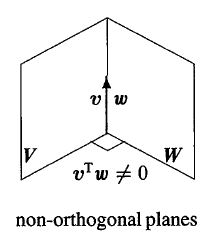
\includegraphics{week5/orthogonality}
\caption{Orthogonality is impossible when $\dim\bm U+\dim\bm V>\dim(\bm U\cup\bm V)$}
\end{figure}
\end{example}
\begin{remark}
When a vector is in two orthogonal subspaces, it \textit{must} be zero. It is \emph{perpendicular} to
itself. 
\\The reason is clear: this vector $\bm u\in\bm U$ and $\bm u\in\bm V$, so $\inp{\bm u}{\bm u}=0$. It has to be zero vector.
\end{remark}
If two subspaces are perpendicular, their basis must be ind.
\begin{theorem}
Assume $\{u_1,\dots,u_k\}$ is the basis for $\bm U$, $\{v_1,\dots,v_l\}$ is the basis for $\bm V.$ If $\bm U\perp\bm V$ ($u_i\perp v_j$ for $\forall i,j$), then $u_1,u_2,\dots,u_k,v_1,v_2,\dots,v_l$ must be ind.
\end{theorem}
\begin{proof}
Suppose there exists $\{\alpha_1,\dots,\alpha_k\}$ and $\{\beta_1,\dots,\beta_l\}$ such that
\[
\alpha_1u_1+\dots+\alpha_ku_k+\beta_1v_1+\dots+\beta_lv_l=\bm 0
\]
then equibalently,
\[
\alpha_1u_1+\dots+\alpha_ku_k=-(\beta_1v_1+\dots+\beta_lv_l)
\]
Then we set $\bm w=\alpha_1u_1+\dots+\alpha_ku_k$, obviously, $\bm w\in\bm U$ and $\bm w\in\bm V$.\\ Hence it must be zero (This is due to remark above). Thus we have
\begin{gather*}
\alpha_1u_1+\dots+\alpha_ku_k=\bm 0\\
\beta_1v_1+\dots+\beta_lv_l=\bm 0.
\end{gather*}
Due to the independence, we have $\alpha_i=0$ and $\beta_j=0$ for $\forall i,j$. 
\end{proof}
\begin{corollary}
If $\{u_1,u_2,\dots,u_k,v_1,v_2,\dots,v_l\}\in\bm W$, then $\dim(\bm W)\ge\dim(\bm U)+\dim(\bm V)$.\\ Note that $\bm U\cup\bm V\subset\bm W$.
\end{corollary}
For subspaces $\bm U$ and $\bm V\in\mathbb{R}^{n}$, if $\mathbb{R}^{n}=\bm U\cup\bm V$, and moreover, $n=\dim(\bm U)+\dim(\bm V)$, then we say $\bm V$ is the \emph{orthogonal complement} of $\bm U$.
\begin{definition}[orthogonal complement]
For subspaces $\bm U$ and $\bm V\in\mathbb{R}^{n}$, if $\dim(\bm U)+\dim(\bm V)=n$ and $\bm U\perp\bm V$, then we say $\bm V$ is the \emph{orthogonal complement} of $\bm U$. And we denote $\bm V$ as $\bm U^{\perp}$.\\
Moreover, $\bm V=\bm U^{\perp}\Longleftrightarrow\bm V^{\perp}=\bm U$.
\end{definition}
\begin{example}
Suppose $\bm U\cup\bm V=\mathbb{R}^{3}$, $\bm U=\Span\{\bm e_1,\bm e_2\}$. If $\bm V$ is the orthogonal complement of $\bm U$, then $\bm V=\Span\{\bm e_3\}$. \\Moreover, $\bm U$ could also be expressed as $\Span\left\{\begin{pmatrix}
1\\1\\0
\end{pmatrix},\begin{pmatrix}
0\\1\\0
\end{pmatrix}\right\}$.
\end{example}
\emph{Example:}\\
Next let's show the nullspace is the orthogonal complement of the row space. (In $\mathbb{R}^{n}$).
Suppose $\bm A$ is a $m\times n$ matrix.
\begin{itemize}
\item
Firstly, we show $\dim(N(\bm A))+\dim(C(\bm A\trans))=\dim(N(\bm A)\cup C(\bm A\trans))=\dim(\mathbb{R}^{n})=n$:\\
We know $\dim(N(\bm A))=n-r$, where $r=\rank(\bm A)$. And $r=C(\bm A\trans))$.\\ Hence $\dim(N(\bm A))+\dim(C(\bm A\trans))=n$.
\item
Then we show $N(\bm A)\perp C(\bm A\trans)$:\\
For any $x\in N(\bm A)$, if we set $\bm A=\begin{bmatrix}
a_1\\a_2\\\vdots\\a_m
\end{bmatrix}$, then we obtain:
\[
\bm{Ax}=\begin{bmatrix}
a_1\\a_2\\\vdots\\a_m
\end{bmatrix}\begin{bmatrix}
\bm x
\end{bmatrix}=\begin{bmatrix}
0\\0\\\vdots\\0
\end{bmatrix}
\]
Hence \textit{every row has a zero product with} $x$. In other words, $\inp{a_i}{x}=0$ for $\forall i\in\{1,2,\dots,m\}$.\\
Hence for any $y=\sum_{i=1}^m\alpha_ia_i\in C(\bm A\trans)$, we obtain:
\[
\begin{aligned}
\inp{x}{y}&=\inp{y}{x}=\inp{\sum_{i=1}^m\alpha_ia_i}{x}\\
&=\sum_{i=1}^{m}\alpha_i\inp{a_i}{x}=0.
\end{aligned}
\]
Hence $x\perp y$ for $\forall x\in N(\bm A)$ and $y\in C(\bm A\trans)$.\\
\end{itemize}
Hence $N(\bm A)^{\perp}=C(\bm A\trans)$.\\
If we applying this equation to $\bm A\trans$, then we have $N(\bm A\trans)^{\perp}=C(\bm A)$. 
\enlargethispage{1cm}
\begin{theorem}[Fundamental theorem for linear alegbra, part 2]\qquad\\
\emph{$N(\bm A)$ is the orthogonal complement of the row space $C(\bm A\trans)$ (in $\mathbb{R}^{n}$).}\\
\emph{$N(\bm A\trans)$ is the orthogonal complement of the row space $C(\bm A)$ (in $\mathbb{R}^{m}$).}
\end{theorem}
\newpage
\begin{corollary}
$\bm{Ax}=\bm b$ is solvable if and only if $\bm y\trans\bm A=\bm 0$ implies $\bm y\trans\bm b$=0.
\end{corollary}
\begin{proof}\qquad\\
$\bm{Ax}=\bm b$ is solvable.
$\Longleftrightarrow$
$\bm b\in C(\bm A)$.
$\Longleftrightarrow$
$\bm b\in N(\bm A\trans)^{\perp}$\\
$\Longleftrightarrow$
$\bm y\trans\bm b=0$ for $\forall y\in N(\bm A\trans)$
$\Longleftrightarrow$
$\bm y\trans\bm A=\bm 0$ implies $\bm y\trans\bm b$=0.
\end{proof}
The Inverse Negative Propositions is more important:
\begin{corollary}
$\bm{Ax}=\bm b$ has no solution if and  and only if $\exists \bm y$ s.t. $\bm y\trans\bm A=0$ and $\bm y\trans\bm b\ne 0$.
\end{corollary}
\begin{remark}
\begin{theorem}\label{theorem_12.3}
$\bm{Ax}\ge\bm b$ has no solution if and only if $\exists \bm y\ge\bm 0$ such that $\bm y\trans\bm A=\bm 0$ and $\bm y\trans\bm b\ge \bm 0$.
\end{theorem}
$\bm y\trans\bm A=0$ requires exists one linear combination of the row space to be zero.
\begin{proof}[Necessity case.]
Suppose $\exists \bm y\ge\bm 0$ such that $\bm y\trans\bm A=\bm 0$ and $\bm y\trans\bm b\ge \bm 0$. And we assume there exists $x^{*}$ such that $\bm Ax^{*}\ge\bm b$. By postmultiplying $\bm y\trans$ we have 
\[\bm y\trans\bm Ax^{*}\ge\bm y\trans\bm b>\bm 0
\implies 
\bm 0>\bm 0.
\]
which is a contradiction!
\end{proof}
The complete proof for this theorem is not required in this course.
\end{remark}
\begin{example}
Given the system 
\begin{equation}
\begin{aligned}
x_1+x_2&\ge1\\
-x_1&\ge-1\\
-x_2&\ge2
\end{aligned}
\end{equation}
Eq(1)$\x$1+Eq(2)$\x$1+Eq(3)$\x$1 gives
\[
0\ge 2
\]
which is a contradiction!\\
So the key idea of theorem (\ref{theorem_12.3}) is to construct a linear combination of row space to let it become zero. Then if the right hand is larger than zero, then this system has no solution.
\end{example}
\begin{remark}
\begin{corollary}
If $\bm A=\bm A\trans$, then $N(\bm A\trans)^{\perp}=C(A)=C(\bm A\trans)=N(\bm A)$.
\end{corollary}
\begin{corollary}\label{corollary_12.5}
The system $\bm{Ax}=\bm b$ may not have a solution, but $\bm A\trans\bm A\bm x=\bm A\trans\bm b$ always have at least one solution for $\forall\bm b$.
\end{corollary}
\begin{proof}
Since $\bm A\trans\bm A$ is symmetric, we have $C(\bm A\trans\bm A)=C(\bm A\bm A\trans)$. You can check by yourself that $C(\bm A\bm A\trans)=C(\bm A\trans)$.
Hence $C(\bm A\trans\bm A)=C(\bm A\trans)$.\\
For any vector $\bm b$ we have $\bm A\trans\bm b\in C(\bm A\trans)\implies\bm A\trans\bm b\in C(\bm A\trans\bm A)$, which means there exists a linear combination of the columns of $\bm A\trans\bm A$ that equals to $\bm b$.\\
Equivalently, there exists a solution to $\bm A\trans\bm A\bm x=\bm A\trans\bm b$.
\end{proof}
\begin{corollary}\label{corollary_12.6}
$\bm A\trans\bm A$ is invertible if and only if columns of $\bm A$ are ind.
\end{corollary}
\begin{proof}
We have shown that $C(\bm A\trans\bm A)=C(\bm A\trans)$.\\ Hence $C(\bm A\trans\bm A)^{\perp}=C(\bm A\trans)^{\perp}\implies N(\bm A\trans\bm A)=N(\bm A)$.\\
$\bm A$ has ind. columns
$\Longleftrightarrow$
$N(\bm A)=\{\bm 0\}$
$\Longleftrightarrow$
$N(\bm A\trans\bm A)=\{\bm 0\}$
$\Longleftrightarrow$
$\bm A\trans\bm A$ is invertible.
\end{proof}
\end{remark}
\subsection{Least Squares Approximations}
$\bm{Ax}=\bm b$ often has no solution, if so, what should we do?\\
We cannot always get the error $\bm e=\bm b-\bm{Ax}$ down to zero, so we want to use least square method to minimize the error. In other words, our goal is to
\[
\min_{\bm x}\bm e^2=\min_{\bm x}\|\bm{Ax}-\bm b\|^2=\sum_{i=1}^{m}(a_i\trans\bm x-b_i)^2
\]
where $\bm A=\begin{bmatrix}
a_1\\a_2\\\vdots\\a_m
\end{bmatrix}$ and $\bm b=\begin{bmatrix}
b_1\\b_2\\\vdots\\b_m
\end{bmatrix}$.\\
The minimizer $\bm x$ is called \emph{linear least squares solution}.
\subsubsection{Matrix Calculus}
Firstly, you should know some basic calculus knowledge for matrix:
\begin{itemize}
\item
$\frac{\partial(f\trans g)}{\partial x}=\frac{\partial f(x)}{\partial x}g(x)+\frac{\partial g(x)}{\partial x}f(x)$
\end{itemize}
Example:
\begin{itemize}
\item
$\frac{\partial(a\trans \bm x)}{\partial \bm x}=a$
\item
$\frac{\partial(a\trans \bm A\bm x)}{\partial \bm x}=\frac{\partial((\bm A\trans a)\trans\bm x)}{\partial \bm x}=\bm A\trans a$
\item
$\frac{\partial(\bm A\bm x)}{\partial \bm x}=\bm A\trans$
\item
$\frac{\partial(\bm x\trans\bm A\bm x)}{\partial \bm x}=\bm A\bm x+\bm A\trans\bm x$
\end{itemize}
Thus, in order to minimize $\|\bm{Ax}-\bm b\|^2=(\bm{Ax}-\bm b)\trans(\bm{Ax}-\bm b)$, we only need to let its \emph{partial derivative} with respect to $\bm x$ to be \emph{zero.} (Since its second derivative is non-negative, we will talk about it in detail in other courses.) Hence we have
\[\begin{aligned}
\frac{\partial (\bm{Ax}-\bm b)\trans(\bm{Ax}-\bm b)}{\partial \bm x}&=\frac{\partial(\bm{Ax}-\bm b)}{\partial \bm x}(\bm{Ax}-\bm b)+\frac{\partial(\bm{Ax}-\bm b)}{\partial \bm x}(\bm{Ax}-\bm b)=2\frac{\partial(\bm{Ax}-\bm b)}{\partial \bm x}(\bm{Ax}-\bm b)\\
&=2(\frac{\partial(\bm A\bm x)}{\partial \bm x}-\frac{\partial(\bm b)}{\partial \bm x})(\bm{Ax}-\bm b)\\
&=2\bm A\trans(\bm{Ax}-\bm b)=\bm 0.
\end{aligned}
\]
Or equivalently, 
\[
\bm A\trans\bm{Ax}=\bm A\trans\bm b.
\]
According to corollary (\ref{corollary_12.5}), this equation always exists a solution. And this equation is called \emph{normal equation}.
\begin{theorem}\label{theorem_12.4}
The partial derivatives of $\|\bm{Ax}-\bm b\|^2$ are \emph{zero} when $\bm A\trans\bm{Ax}=\bm A\trans\bm b.$
\end{theorem}
\subsubsection{Fit a stright line}
Given a collection of data $(\bm x_i,y_i)$ for $i=1,\dots,m$, we can fit the model parameters:
\[
\left\{
\begin{aligned}
y_1&=a_0+a_1x_{1,1}+a_2x_{1,2}+\dots+a_nx_{1,n}+\varepsilon_1\\
y_2&=a_0+a_1x_{2,1}+a_2x_{2,2}+\dots+a_nx_{2,n}+\varepsilon_2\\
\vdots\\
y_m&=a_0+a_1x_{m,1}+a_2x_{m,2}+\dots+a_nx_{m,n}+\varepsilon_m
\end{aligned}
\right.
\]
Our fit line is 
\[
\hat y=a_0+a_1x_1+a_2x_2+\dots+a_nx_n
\]
In \textit{compact matrix form}, we have
\[
\begin{bmatrix}
y_1\\y_2\\\vdots\\y_n
\end{bmatrix}
=\begin{bmatrix}
1&x_{1,1}&x_{1,2}&\dots&x_{1,n}\\
1&x_{2,1}&x_{2,2}&\dots&x_{2,n}\\
\vdots&\vdots&&&\\
1&x_{m,1}&x_{m,2}&\dots&x_{m,n}\\
\end{bmatrix}\begin{bmatrix}
a_0\\a_1\\a_2\\\vdots\\a_{n}
\end{bmatrix}+\begin{bmatrix}
\varepsilon_1\\\varepsilon_2\\\vdots\\\varepsilon_m
\end{bmatrix}
\]
Or equivalently, we have 
\[
\bm y=\bm{Ax}+\bm \varepsilon
\]
where $\bm A =\begin{bmatrix}
1&x_{1,1}&x_{1,2}&\dots&x_{1,n}\\
1&x_{2,1}&x_{2,2}&\dots&x_{2,n}\\
\vdots&\vdots&&&\\
1&x_{m,1}&x_{m,2}&\dots&x_{m,n}\\
\end{bmatrix}_{m\times (n+1)}$, $\bm x=\begin{bmatrix}
a_0\\a_1\\a_2\\\vdots\\a_{n}
\end{bmatrix}_{(n+1)\times 1}$, $\bm \varepsilon=\begin{bmatrix}
\varepsilon_1\\\varepsilon_2\\\vdots\\\varepsilon_m
\end{bmatrix}_{m\times 1}$.\\
Our goal is to minimize $\|\hat{\bm y}-\bm y\|^2=\|\bm{Ax}-\bm y\|^2$. Then by theorem (\ref{theorem_12.4}), we only need to sovle $\bm A\trans\bm A\bm x=\bm A\trans\bm y$.
\subsection{Projections}
In corollary (\ref{corollary_12.6}), we know that if $\bm A$ has ind. columns, then $\bm A\trans\bm A$ is invertible. On this condition, the normal equation $\bm A\trans\bm A\bm x=\bm A\trans\bm b$ has unique solution $\bm x^{*}=(\bm A\trans\bm A)^{-1}\bm A\trans\bm b$.\\
Thus the error $\bm b-\bm A\bm x^{*}$ is minimum. And $\bm A\bm x^{*}=\bm A(\bm A\trans\bm A)^{-1}\bm A\trans\bm b$ \emph{approximately} equals to $\bm b$. \\
\begin{itemize}
\item
If $\bm b$ and $\bm{A}\bm x^{*}$ are exactly in the same space, then $\bm{A}\bm x^{*}=\bm b$.
\item
Otherwise, just as the Figure (\ref{figure_12.2}) shown, $\bm A\bm x^{*}$ is the projection of $\bm b$ to subspace $C(\bm A)$.
\end{itemize}
\begin{figure}[H]\centering
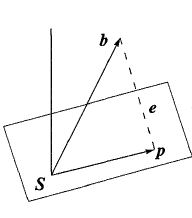
\includegraphics{week5/projection}
\caption{The projection of $\bm b$ onto a subspace $C(\bm A)$.}\label{figure_12.2}\end{figure}
\begin{definition}[Projection]
The projection of $\bm b$ onto the subspace $C(\bm A)$ is denoted as $\Proj_{C(\bm A)}(\bm b)$.
\end{definition}
\begin{definition}[Projection matrix]
Given $\bm A\bm x^{*}=\bm A(\bm A\trans\bm A)^{-1}\bm A\trans\bm b=\Proj_{C(\bm A)}(\bm b)$. Since $[\bm A(\bm A\trans\bm A)^{-1}\bm A\trans]\bm b$ is the projection of $\bm b$, we call $\bm P=\bm A(\bm A\trans\bm A)^{-1}\bm A\trans$ as \emph{projection matrix}.
\end{definition}
\begin{definition}[Idempotent]
Let $\bm A$ be a \emph{square} matrix that satisfies $\bm A=\bm A\bm A$, then $\bm A$ is called a \emph{idempotent} matrix.
\end{definition}
Let's show the projection matrix is \textit{idempotent}:\\
\[
\begin{aligned}
\bm P^{2}&=\bm A(\bm A\trans\bm A)^{-1}\bm A\trans\bm A(\bm A\trans\bm A)^{-1}\bm A\trans\\
&=\bm A(\bm A\trans\bm A)^{-1}(\bm A\trans\bm A)(\bm A\trans\bm A)^{-1}\bm A\trans\\
&=\bm A(\bm A\trans\bm A)^{-1}\bm A\trans=\bm P.
\end{aligned}
\]
\subsubsection{Observations}
\begin{itemize}
\item
If $\bm b\in C(\bm A)$, then $\exists \bm x$ s.t. $\bm{Ax}=\bm b$. Moreover, the projection of $\bm b$ is exactly $\bm b$:
\[
\begin{aligned}
\bm{Pb}&=\bm A(\bm A\trans\bm A)^{-1}\bm A\trans(\bm b)\\
&=\bm A(\bm A\trans\bm A)^{-1}\bm A\trans(\bm{Ax})\\
&=\bm A(\bm A\trans\bm A)^{-1}(\bm A\trans\bm A)\bm x\\
&=\bm{Ax}=\bm b.
\end{aligned}
\]
\item
Assume $\bm A$ has only one column, say, $\bm a$. Then we have
\[\begin{aligned}
\bm x^{*}&=(\bm A\trans\bm A)^{-1}\bm A\trans\bm b=\frac{\bm a\trans\bm b}{\bm a\trans\bm a}\\
\bm A\bm x^{*}&=\bm{Pb}=\bm A(\bm A\trans\bm A)^{-1}\bm A\trans(\bm b)=\frac{\bm a\trans\bm b}{\bm a\trans\bm a}\times\bm a=\frac{\bm a\trans\bm b}{\|\bm a\|^2}\times\bm a
\end{aligned}
\]
More interestingly, 
\[\frac{\bm a\trans\bm b}{\|\bm a\|^2}\times\bm a=\frac{\|\bm a\|\|\bm b\|\cos\theta}{\|\bm a\|^2}\times\bm a=\|\bm b\|\cos\theta\times\frac{\bm a}{\|\bm a\|}\]
which is the projection of $\bm b$ onto a line $\bm a$. (Shown in figure below.)
\begin{figure}[H]
\centering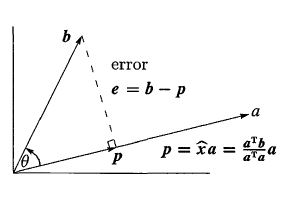
\includegraphics[width=10cm]{week5/projection_line}
\caption{The projection of $\bm b$ onto a line $\bm a$.}
\end{figure}
More generally, we can write the projection of $\bm b$ as:
\[
\Proj_{\bm a}(\bm b)=\frac{\inp{\bm a}{\bm b}}{\inp{\bm a}{\bm a}}\bm a
\]
Look at the figure above! The error is $\bm b-\Proj_{\bm a}(\bm b)$, which is obviously perpendicular to $\bm a$. And $\bm b-\Proj_{\bm a}(\bm b)\in\Span\{\bm a,\bm b\}$.\\
If we define $\bm b'=\bm b-\Proj_{\bm a}(\bm b)$, then it's easy to check $\Span\{\bm a,\bm b'\}=\Span\{\bm a,\bm b\}$ and $\bm a\perp\bm b'$. Hence we convert a basis to another basis such that the elements are orthogonal to each other. We will discuss it in detail in next lecture. 
\end{itemize}








